%-*- coding: utf-8 -*-
\documentclass[11pt,a4paper,oneside]{book} %twoside,openright
%-*- coding: utf-8 -*-
\usepackage[utf8]{inputenc}
\usepackage[T1]{fontenc}
\usepackage{graphicx}%pour insérer images et pdf entre autres
	\graphicspath{{images/}}%pour spécifier le chemin d'accès aux images
\usepackage[left=2.5cm,right=2.5cm,top=2.5cm,bottom=2.5cm]{geometry}%réglages des marges du document selon vos préférences ou celles de votre établissemant
\usepackage[Lenny]{fncychap}%pour de jolis titres de chapitres voir la doc pour d'autres styles.
\usepackage{babel}
\usepackage[babel=true]{csquotes} % csquotes va utiliser la langue définie dans babel

\usepackage{fancyhdr}%pour les entêtes et pieds de pages
	\setlength{\headheight}{14.2pt}% hauteur de l'entête
        \chead{\textbf{ARROSAGE}}
        \lhead{}
        \rhead{}
	\cfoot{Formation Ingénieur Informatique en alternance - Deuxième année}
	\lfoot{\textbf{CNAM}}%
  	\rfoot{\textbf{\thepage/\pageref{LastPage}}}
 	\renewcommand{\headrulewidth}{0.4pt}%trait horizontal pour l'entête
  	\renewcommand{\footrulewidth}{0.4pt}%trait horizontal pour les pieds de pages

\usepackage[french]{nomencl}
\makenomenclature
\usepackage{hyperref}


\begin{document}
\let\cleardoublepage\clearpage
\frontmatter
\pagestyle{front}
%-*- coding: utf-8 -*-
%\phantomsection
\begin{titlepage}
\color[RGB]{91, 155, 213}
\parindent=0pt

\hrulefill
\begin{center}\bfseries\Huge
PROJET SMART WATER
\end{center}
\hrulefill

%\begin{center}\bfseries\Large
% sous-titre
%\end{center}

\begin{center}
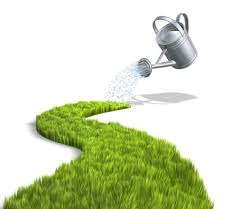
\includegraphics[scale=1.0]{images/arrosage.jpg}%
\end{center}

\vspace*{1cm}
\begin{center}\bfseries\Large
Samir HADJOUTRIOS

Elzbieta IGUAL

Jérôme GARCIA

Jean-Félix BENITEZ

Nicolas SYMPHORIEN
\end{center}

\vspace*{\stretch{2}}

CNAM \hspace*{\stretch{1}} Formation en alternace

Ingénieur Informatique \hspace*{\stretch{1}} Deuxième année

\end{titlepage}

\thispagestyle{empty}                        % pour la page de garde toute blanche

\mainmatter
\pagestyle{main}
%-*- coding: utf-8 -*-
\begin{center}\bfseries\Huge
    Feuille de suivi des évolutions
\end{center}
\begin{longtable}{|c|p{3.5cm}|c|p{9cm}|}
  \hline
  Indice & Éléments concernés & Date & Raison et nature de l'évolution \\ \endfirsthead \hline
  Indice & Éléments concernés & Date & Raison et nature de l'évolution \\ \endhead \hline
  - & Toutes les pages & 11/02/2018 & Création du document\\
   & & & \\
   & & & \\
   & & & \\
   & & & \\
   & & & \\
   & & & \\
   & & & \\
   & & & \\
   & & & \\
   & & & \\
   & & & \\
   & & & \\
   & & & \\
   & & & \\
   & & & \\
   & & & \\
   & & & \\
   & & & \\
   & & & \\
   & & & \\
   & & & \\
   & & & \\
   & & & \\
   & & & \\
   & & & \\
   & & & \\
   & & & \\
   & & & \\
   & & & \\
   & & & \\
   & & & \\
   & & & \\
   & & & \\
   & & & \\
   & & & \\
   & & & \\
   & & & \\
   & & & \\
   & & & \\
   & & & \\
   & & & \\
   & & & \\
   & & & \\
   & & & \\
   & & & \\
   & & & \\
   & & & \\ \hline
\end{longtable}

\tableofcontents
\listoffigures
\listoftables
%-*- coding: utf-8 -*-
\textcolor[RGB]{46, 116, 181}{\chapter{Présentation}}
\section{Objet du document}
Ce document est le rapport du travail fait sur le projet de système d'arrosage.

\section{Domaine d'application}
Formation du CNAM en ingénieur informatique deuxième année.

\section{Description du document}
Les trois premiers chapitres définissent le contenu de ce document~; les chapitres suivants décrivent le travail fait sur ce projet.

\section{Emplacement du document}
\href{https://github.com/garje31/arrosage-auto/}{\emph{https://github.com/garje31/arrosage-auto/}}


%-*- coding: utf-8 -*-
\textcolor[RGB]{46, 116, 181}{\chapter{Documents}}
\section{documents applicables}
Sans objet.
\section{documents de référence}
\setenumerate{font=\bfseries, label=R\arabic*}
Sans objet.
%\begin{enumerate}
%\item\label{...} ...
%
%\url{}
%\end{enumerate}
\setenumerate{}

%-*- coding: utf-8 -*-
\textcolor[RGB]{46, 116, 181}{\chapter{Terminologie}}
\section{Abréviations}
\rowcolors{1}{red!26!green!29!blue!31!}{}
\begin{table}[!h]
\begin{tabular}{p{2.5cm}p{13.5cm}}
  &\\
  &\\
  &\\
  &\\
  &\\
  &\\
  &\\
\end{tabular}
\caption{abréviations}
\end{table}

\section{Glossaire}
\begin{table}[!h]
\begin{tabular}{lp{13.5cm}}
  %\textbf{...} & ... \\
  &\\
  &\\
  &\\
  &\\
  &\\
\end{tabular}
\caption{glossaire}
\end{table}
\printglossaries

%-*- coding: utf-8 -*-
\textcolor[RGB]{46, 116, 181}{\chapter{Analyse Contextuelle}}
L'arrosage d'un jardin ou de plantes dans un espace de vente est une tâche qui doit être faite quotidiennement du printemps à l'automne.
Quand elle n'est pas faite manuellement, c'est un réseau de tuyaux d'arrosages proportionnel au nombre de plantes qui est mis en oeuvre.
Ce réseau doit être modifié à chaque fois que l'on déplace 1 ou plusieurs plantes. Il doit être vérifié et remis en état à chaque début de saison.
Le système proposé ici permet l'arrosage des plantes de la même façon que le ferait un être humain; sans réseau de tuyaux.

\jerome{\section{Problème} 
Le réseau de tuyaux doit être entretenu impose des coûts proportionnels à sa taille. 
Cet entretien doit être fait plusieurs fois par semaine, et l'arrosage des plantes efectué quotidiennement. Il faut donc embaucher du personnel qualifié 
pour répondre au problème du temps qui, là aussi, est proportionnel à la taille de la pépinière ou du jardin. }

\samir
{
L'arrosage de plantes dans un jardin est une tâche à réaliser quotidiennement du printemps à l'automne.
Quand elle n'est pas effectuée par un opérateur humain, c'est un réseau de tuyaux et de jets qui s'en charge.
Dans le cas premier cas, le problème tient au coût engendré par le temps conséquent passé à arroser.
Dans le second cas, le problème tient à la plus ou moins grande complexité de sa mise en place, son entretien régulier sous l'action des éléments, son réaménagement obligatoire induite par les déplacements de pots ou la croissance des plantes et enfin, le coté peu esthétique de ce type d'installation.
}

\jeanfelix{Contribution de Jean-Félix.}

\jerome{Contribution de Jérôme.}

\ela{Contribution de Ela.}

\nicolas{Contribution de Nicolas.}

\section{Finalité}
La finalité du système d'arrosage est de veiller à la bonne santé des plantes partout où c'est nécessaire.

\jerome{
Le système proposé contribue à l'entretien des espaces privés et au développement de la faune et de la flore.}

\samir
{
Notre système sera chargé d'arroser les plantes en pots ou en terre des jardins et des pépinières, selon leurs besoins. Il devra répondre aux problèmes de coûts, de complexité, d'entretien et d'inesthétisme des solutions existantes.
}

\section{Conceptualisation}
Les missions du système d'arrosage sont:
\begin{itemize}
\item Arroser les plantes aussi souvent que nécessaire.
\item Détecter la présence d'anomalies: parasites, maladies.
\end{itemize}

\jerome{
\begin{itemize}
\item Arrosage automatique des pépinières et jardins
\item Parcourir une zone non cartographiée
\item Détecter et alerter les problèmes techniques liés au système
\end{itemize}
}

\samir
{
La mission unique du système consiste à arroser les plantes en pots ou en terre des jardins et des pépinières, selon leurs besoins.
}



%-*- coding: utf-8 -*-
\textcolor[RGB]{46, 116, 181}{\chapter{Analyse des exigences}}
\section{Parties prenantes}
\begin{description}
\item[Participantes:] Jardinier, pépiniériste, horticulteur.
\item[Concernées:] ?
\item[Impactées:] Visiteurs, clients.
\end{description}

\section{Besoins}
\begin{enumerate}
\item Pouvoir faire un arrosage spécifique à chaque catégorie de plantes; voire à chaque plante.
\item Conditionner l'arrosage aux variations climatiques.
\item Planifier les arrosages, leurs périodicité.
\end{enumerate}

\section{Exigences}


%-*- coding: utf-8 -*-
\textcolor[RGB]{46, 116, 181}{\chapter{Analyse fonctionnelle externe}}
\section{Fonctions de services}

\section{Fonctions internes}

\section{Architecture fonctionnelle}

%-*- coding: utf-8 -*-
\textcolor[RGB]{46, 116, 181}{\chapter{Architecture technique}}
\section{Composants}

\section{Flux}

\section{Comportements}

%\input{E_Realisation/Realisation}

\appendix
\newcommand{\annexe}[1]{%
	\refstepcounter{chapter}%
	\phantomsection%
	\addcontentsline{toc}{chapter}{\appendixname~{\thechapter}: #1}%
	\chapter*{\appendixname~{\thechapter}: #1}}
\annexe{...}

\label{annexeA}

\section{}

\subsection{}

\label{LastPage}
\end{document}
